% Titre : $u_{n+1} = \cos(u_n)$
% Filiere : BCPST
% Difficulte :
% Type : DS, DM
% Categories : info
% Subcategories : 
% Keywords : info




\begin{probleme}[Informatique]
Soit $\suiteu$ la suite définie par $\left\{ \begin{array}{ll} 
u_0&=0\\
u_{n+1} &= \cos(u_n)
\end{array}\right.$

\begin{enumerate}
\item Ecrire une fonction \texttt{suite\_u} qui prend comme paramètre d'entrée un entier $n$ et calcule la valeur de $u_n$ correspondante. 
\item On souhaite étudier le comportement de la suite $\suite{u}$, ou tout du moins de ces premiers termes. Ecrire pour cela un programme qui trace un graphique sur lequel se trouvent les points $(n,u_n)$ pour $n\in \intent{0,20}$.

\begin{minipage}[t]{0.4 \textwidth}
On obtient le graphe suivant
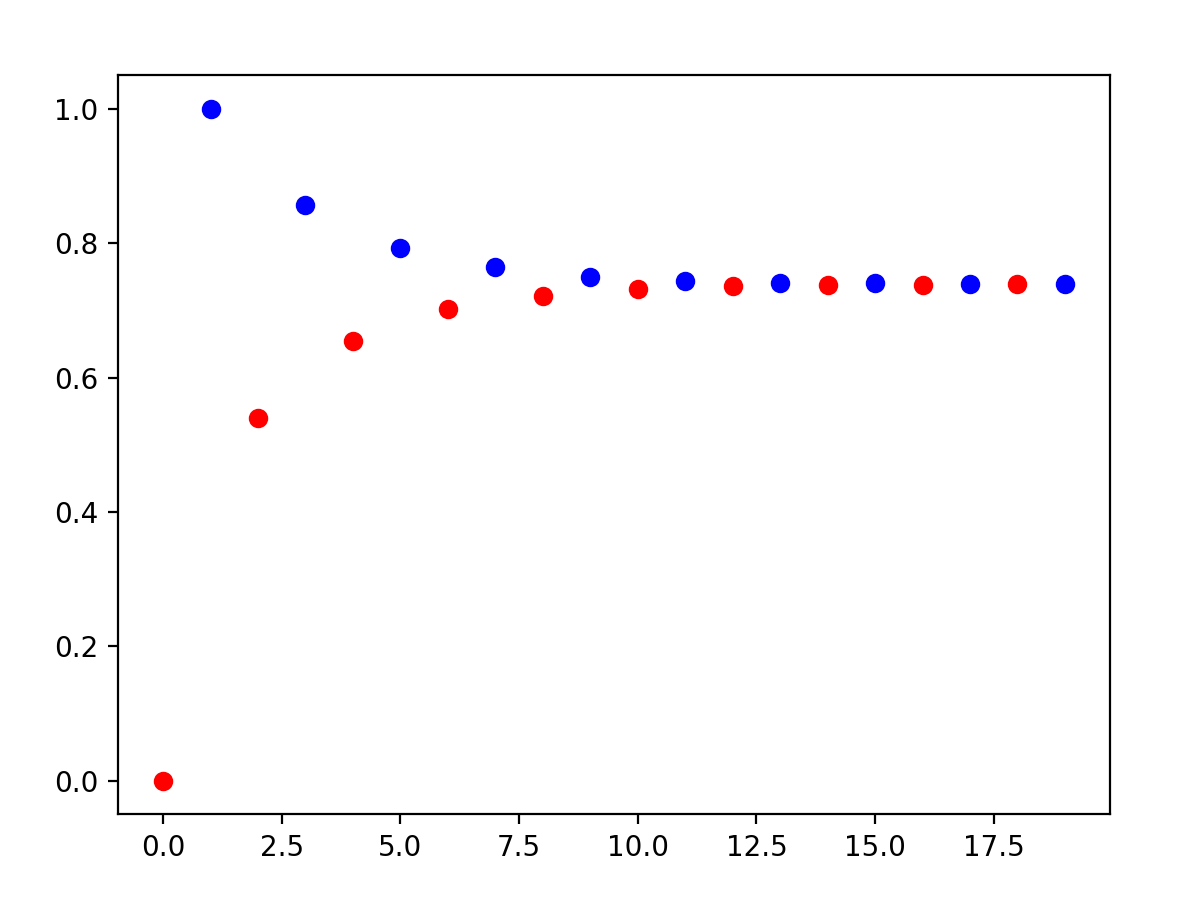
\includegraphics[scale=0.3]{suiteu}

\end{minipage}
\hfill\vline\hfill
\begin{minipage}[t]{0.5 \textwidth}
Les suites $(u_{2n})$ et $(u_{2n+1})$ semblent adjacentes, et converger vers une même limite $\ell$, de sorte que :
$$\lim_{n\tv +\infty} u_n =\ell.$$
En particulier, $\ell$ semble toujours appartenir à l'intervalle d'extrémités $u_n$ et $u_{n+1}$ pour tout entier $n\in \N$, ce qui s'écrit :
$$\forall n\in N, |\ell - u_n| \leq |u_{n+1} - u_n|$$
Nous admettrons tous ces résultats sans démonstration pour la suite. 
\end{minipage}
\item Justifier que le réel $\ell$ satisfait $\ell = \cos(\ell)$ 
\item Proposer un programme permettant de tracer les courbes représentatives des fonctions $f : x\mapsto \cos(x)$ et $g : x \mapsto x$ sur l'intervalle $[0,1]$. \\
Après exécution, ce programme génère le graphe suivant : 
\begin{center}
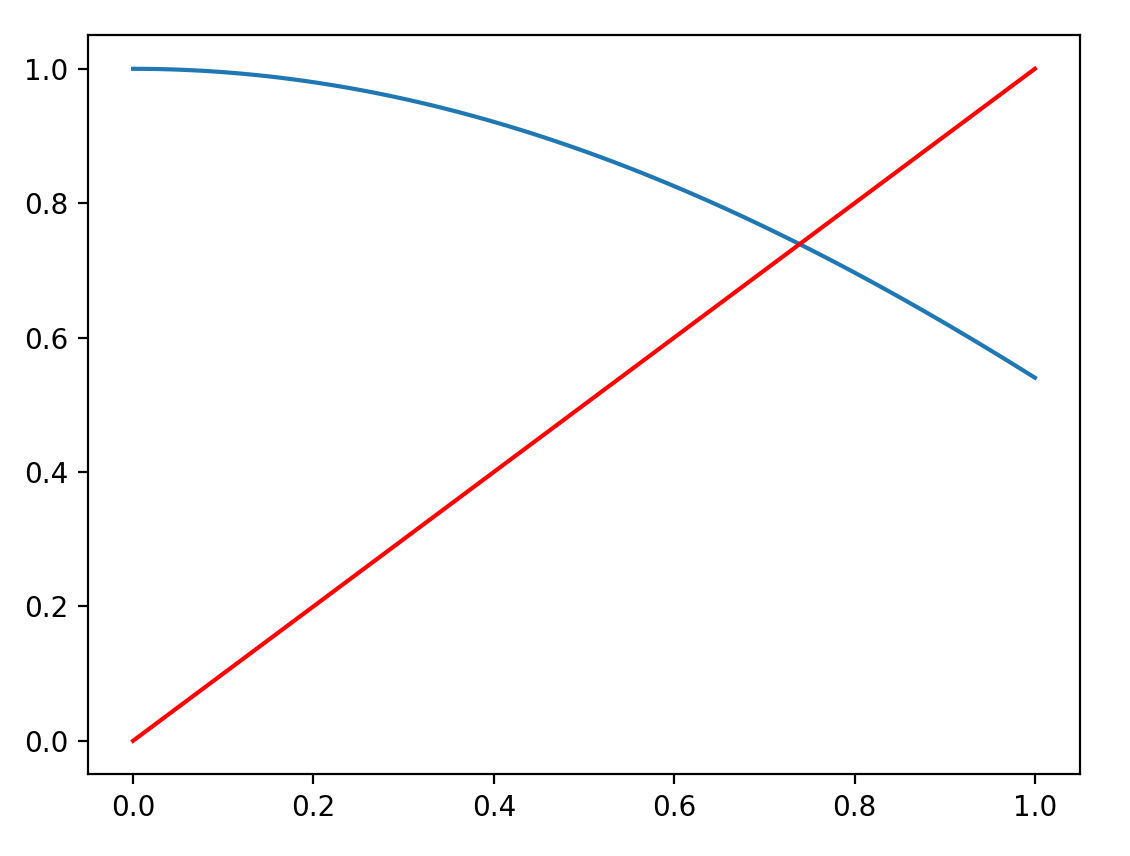
\includegraphics[scale=0.4]{cos}
\end{center}
Déterminer par lecture graphique une valeur approchée de $\ell$. 
\item \begin{enumerate}
\item Ecrire une fonction \texttt{premier\_entier(p)} qui prend comme paramètre d'entrée un entier $p$ et renvoie le plus petit entier tel que $|u_{n+1} - u_n| \leq 10^{-p}$
\item En déduire une fonction $\texttt{approx(p)}$ qui prend comme paramètre d'entrée un entier $p$ et renvoie une valeur approchée de $\ell $ à $\pm 10^{-p}$ prés. 
\end{enumerate}
\item On souhaite déterminer une valeur approchée de $\ell $ par une autre méthode en utilisant un algorithme de dichotomie. On considère pour cela la fonction $h : x \in [0,1] \mapsto x- \cos(x).$
\begin{enumerate}
\item Monter que $h$ s'annule en un unique point de $\alpha \in [0,1]$ et que $\alpha =\ell$. 
\item On suppose avoir défini la fonction $h$ sur Python. Compléter la fonction suivante, qui prend comme paramètre d'entrée un réel $\epsilon>0$ et qui renvoie une valeur approchée de $\ell$ à $\epsilon $ prés à l'aide de la méthode de la dichotomie. 
\begin{lstlisting}
def dichotomie(epsilon):
    a=0
    b=1

    while      >    :
        milieu = (a+b)/2
        if h(milieu)*h(a)<0:
            
        else:
            
    return(a)
\end{lstlisting}


\end{enumerate}
\end{enumerate}




\end{probleme}

\begin{correction}
3 - Comme $u_n$ converge vers $\ell$ par unicité de la limite $u_{n+1}$ converge vers $\ell$. Comme $\cos$ est continue sur $\R$ on a 
$lim_{n\tv\infty} \cos(u_n) = \cos(\ell)$. Ainsi $\ell =\cos(\ell)$\\
4- $\ell \simeq 0.8$\\
6-a C'est une application du théorème de la bijection. 
$h$ est continue et dérivable sur $[0,1]$ et $h'(x) = 1+sin(x) >0$ donc $h$ est strictement croissante. $h(0)=-1$ et $h(1)= 1-\cos(1)>0 $ donc d'après le théorème de la bijection il existe un unique $\alpha \in [0,1]$ tel que $h(\alpha) =0$. 
$\alpha$ vérifie donc $\alpha-\cos(\alpha)=0$ cad $\alpha =\cos(\alpha)$ par unicité de la solution sur l'intervalle $[0,1]$ il est égale à $\ell$. 

\end{correction}